\documentclass[pscyr]{hedwork}
\usepackage[russian]{babel}
\usepackage[derivative,root,shortcuts,environments]{hedmaths}

\faculty{Факультет электроники и вычислительной техники}
\department{<<Физика>>}
\subject{Термодинамика и статистическая физика}
\variant{18}
\student[m]{студент группы Ф-469 \\ Чечеткин И. А.}
\teacher[m]{профессор, д. физ.-мат. н. \\ Крючков С. В.}

\newcommand{\vg}{{\vphantom{\gamma}}}

\renewcommand{\labelenumi}{\asbuk{enumi})}

\makeatletter
  \@addtoreset{equation}{task}
  \renewcommand{\theequation}{\thetask.\arabic{equation}}
\makeatother

\usepackage{graphicx}
\graphicspath{{images/dsk_}}

\begin{document}

  \maketitle

  \begin{task}{8 (ТД)}{
    Вычислите критические параметры \( V_\text{к} \), \( p_\text{к} \),
    \( T_\text{к} \) газа Ван-дер-Ваальса, выражая их через постоянные
    \( a \) и \( b \) для этого газа.
  }

    Уравнение Ван-дер-Ваальса:
    \[
      \left(P + \frac{a}{V^2}\right)\Bigl(V - b\Big) = RT.
    \]

    Домножим на \( V^2 \) и раскроем скобки:
    \begin{equation}
      PV^3 - (RT + Pb)V^2 + aV - ab = 0.
      \label{eq:1.1}
    \end{equation}

    По определению критических параметров, это уравнение можно записать в виде:
    \begin{gather}
      P_\text{к} (V - V_\text{к})^3 = 0, \text{ раскрывая куб, получим:}
        \nonumber \\
      P_\text{к} (V^3 - 3V^2 V_\text{к} + 3V V_\text{к}^2 - V_\text{к}^3),
        \text{ или,}\nonumber \\
      P_\text{к} V^3 - 3P_\text{к} V^2 V_\text{к} + 3P_\text{к}^\vg V
        V_\text{к}^2 - P_\text{к}^\vg V_\text{к}^3 = 0. \label{eq:1.2}
    \end{gather}

    Сравнивая \eqref{eq:1.2} с \eqref{eq:1.1} видно, что:
    \[
      ab = P_\text{к}^\vg V_\text{к}^3; \quad
        3P_\text{к}^\vg V_\text{к}^2 = a; \quad
        RT_\text{к} + P_\text{к}b = 3P_\text{к} V_\text{к}.
    \]

    Подставляя второе равенство в первое, находим, что \(  V_\text{к} = 3b \).

    Подставляя это обратно во второе равенство, получим, что
    \( P_\text{к} = a / (27b^2) \).

    Подставляя \( P_\text{к} \) и \( V_\text{к} \) в третье равенство, получим,
    что \( T_\text{к} = 8a / (27 Rb) \).

    Таким образом,
    \(
      \ds P_\text{к} = \frac{a}{27b^2},\ V_\text{к} = 3b,\
        T_\text{к} = \frac{8}{27}\frac{a}{Rb}
    \).

  \end{task}

  \begin{task}{88 (ТД)}{
    Воздух сжимается по политропе, описываемой уравнением
    \( pV^{1,45} = \const \). Как при этом будет изменяться его температура?
  }

    Поскольку воздух можно считать идеальным газом, то его состояние
    описывается уравнением Менделеева--Клапейрона:
    \[
      PV = \nu RT, \quad P = \nu R\frac{T}{V}.
    \]

    Подставляя \( P \) в уравнение политропы, получим
    \[
      PV^{1,45} = TV^{0,45} = \const.
    \]

    Поскольку газ сжимается, то объем уменьшается, а температура, следовательно,
    возрастает: \( \D T > 0 \).

  \end{task}

  \begin{task}{130 (ТД)}{
    Найдите выражение для к.~п.~д. карбюраторного четырехтактного двигателя
    внутреннего сгорания, работающего по циклу Отто, состоящему из двух
    адиабатических и двух изохорических процессов. Параметром цикла является
    величина \( \eps = V_1 / V_2 \)~-- степень сжатия горючей смеси, которую
    можно считать идеальным газом.
  }

    \begin{figure}[h!]
      \center
      \begin{minipage}{.38\textwidth}
        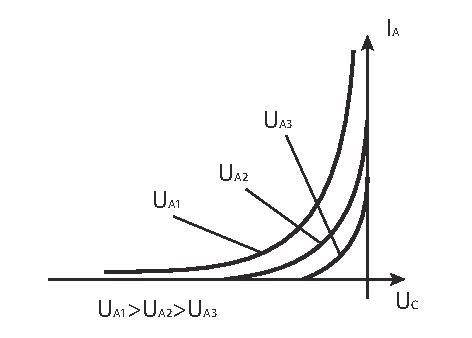
\includegraphics[width=\textwidth]{3}
      \end{minipage} \hfill
      \begin{minipage}{.6\textwidth}
        К.~п.~д. цикла равен:
        \begin{equation}
          \eta = \frac{A}{Q_i} = \frac{Q_i - Q_o}{Q_i}.
          \label{eq:3.1}
        \end{equation}

        Теплота \( Q_i \) поступает при изохорическом процессе \( 2 \to 3 \),
        теплота \( Q_o \) уходит при изохорическом процессе \( 4 \to 1 \).

        Тогда
        \begin{equation}
          Q_i = C_V\nu\D T_{23}, \quad Q_o = C_V\nu\D T_{41},
          \label{eq:3.2}
        \end{equation}
        где \( \D T_{23} = T_3 - T_2 \), \( \D T_{41} = T_4 - T_1 \).
      \end{minipage}
    \end{figure}

    Уравнения состояний 1, 2, 3 и 4:
    \begin{equation}
      P_1 V_1 = \nu RT_1, \quad P_2 V_2 = \nu RT_2, \quad
        P_3 V_2 = \nu RT_3, \quad P_4 V_1 = \nu RT_4.
      \label{eq:3.3}
    \end{equation}

    Уравнения адиабат \( 3 \to 4 \) и \( 1 \to 2 \):
    \begin{equation}
      P_3^\vg V_2^\gamma = P_4^\vg V_1^\gamma, \quad
        P_1^\vg V_1^\gamma = P_2^\vg V_2^\gamma.
      \label{eq:3.4}
    \end{equation}

    Выразим из \eqref{eq:3.3} давления \( P_1 \), \( P_2 \), \( P_3 \) и
    \( P_4 \) и подставим в \eqref{eq:3.4}:
    \[
      T_3^\vg V_2^{\gamma - 1} = T_4^\vg V_1^{\gamma - 1}, \quad
        T_1^\vg V_1^{\gamma - 1} = T_2^\vg V_2^{\gamma - 1}.
    \]

    Тогда \( T_3 = T_4 \bigl(V_1 / V_2\big)^{\gamma - 1} \) и
    \( T_2 = T_1 \bigl(V_1 / V_2\big)^{\gamma - 1} \), откуда
    \( T_3 - T_2 = \bigl(T_4 - T_1\big)\eps^{\gamma - 1} \).

    Подставим это и \eqref{eq:3.2} в \eqref{eq:3.1}:
    \[
      \eta = \frac{\D T_{23} - \D T_{41}}{\D T_{23}} =
        1 - \frac{\D T_{41}}{\D T_{23}} = 1 - \frac{T_4 - T_1}{T_3 - T_2} =
        1 - \frac{T_4 - T_1}{T_4 - T_1}\frac{1}{\eps^{\gamma - 1}} =
        1 - \frac{1}{\eps^{\gamma - 1}}.
    \]

    Таким образом, \( \eta = 1 - 1 / \eps^{\gamma - 1} \).

  \end{task}

  \begin{task}{246 (ТД)}{
    Докажите, что для однородной изотропной системы теплоемкость при постоянном
    давлении равна
    \[
      C_p = T\left[\left(\ppder{I}{S}\right)_{\!\!p}\right]^{-1} \!\!,
    \]
    где \( I \)~-- энтальпия.
  }

    По определению энтальпии:
    \[
      dI = T\,dS + V\,dp.
    \]

    Первая производная по \( S \) от \( I \) при постоянном \( p \):
    \[
      \left(\pder{I}{S}\right)_{\!\!p} = T.
    \]

    Вторая производная:
    \begin{equation}
      \left(\ppder{I}{S}\right)_{\!\!p} = \left(\pder{T}{S}\right)_{\!\!p} =
        T \cdot \left(\frac{\partial T}{T\partial S}\right)_{\!\!p} =
        T \cdot \frac{1}{C_p},
      \label{eq:4.1}
    \end{equation}
    поскольку
    \[
      \frac{\delta Q}{dT} = C; \quad T\,dS = Q.
    \]

    Выражая \( C_p \) из \eqref{eq:4.1}, получим в итоге
    \[
      C_p = T \cdot \left[\left(\ppder{I}{S}\right)\right]^{-1}\!\!.
    \]

  \end{task}

  \begin{task}{321 (СФ)}{
    Для линейного гармонического осциллятора с энергией \( \eps \) вычислить
    фазовый объем \( \Gamma \), ограниченный гиперповерхностью энергии. Оценить
    объем элементарной фазовой ячейки, используя формулу энергетического спектра
    \[
      \eps_n = h\nu \left(n + \frac{1}{2}\right),
    \]
    где \( n = 0, 1, 2, \ldots \).
  }

  \end{task}

  \begin{task}{410 (СФ)}{
    Пользуясь теоремами о равномерном распределении кинетической энергии по
    степеням свободы и о вириале в виде
    \[
      \overline{q_i\pder{H}{q_i}} = \overline{p_i\pder{H}{p_i}},
    \]
    вычислить среднюю энергию линейного гармонического осциллятора.
  }

  \end{task}

  \begin{task}{456 (СФ)}{
    Химический потенциал \( \eta \) бозе-газа определяется равенством
    \[
      \frac{N}{V} = 2\pi(2s + 1)(2mk_0 T)^{3/2} h^{-3}
        \int\lni \frac{\sqrt{z}\,dz}{e^{z - \eta / (k_0 T)} - 1},
    \]
    где \( s \)~-- спин частицы и \( z = \eps / (k_0 T) \). Определить
    температуру бозе-конденсации.
  }

  \end{task}

  \begin{task*}{450 (СФ)}{
    Оценить удельную электронную теплоемкость (на единицу массы) для лития и
    натрия, предполагая, что валентные электроны в обоих случаях можно
    рассматривать как свободные. Плотности лития и натрия равны соответственно
    \( 0,\!534 \) и \( 0,\!97 \) г/см\( ^3 \).
  }

  \end{task*}

\end{document}
